% !TeX root = ../main.tex

\chapter{区块链技术}

\section{区块链系统分类}

区块链技术旨在不可信的开放网络中,维护一个安全可信、不可篡改的公共账本,并以此为基础构建电子 交易、访问控制等应用系统.根据新节点的加入是否需要授权认证,区块链系统可以分为许可链和非许可链两 大类.非许可链通常也称为公有链,不限制节点的加入或退出,任何节点可以访问链上数据、发布交易、以及 参与链上数据的记录,甚至可以尝试发布不合法消息,攻击网络中的其他节点.许可链指区块链网络中节点 的加入网络、记录账本等操作需要经过特定的授权许可与认证.许可链系统又可以根据系统参与方的数量分 为联盟链与私有链,其中联盟链由多方组织加入同一区块链网络中,共同维护区块链账本,记录并执行链上合 约,多方组织可以通过一致的账本建立起联盟成员之间的信任.而私有链通常由一个参与方负责创建和维护, 主要用于记录和管理内部数据,增强数据的安全性、可追溯性. 

本文对比许可链和非许可链两类区块链系统在准入限制、参与方数量、采用的共识算法、应用场景等方面的区别,并总结如表\ref{table:classification} 所示. 

\begin{table}  
\caption{区块链分类}  
\begin{tabularx}{15cm}{X|X|X}
\hline  
名称 & 非许可链 & 许可链 \\ \hline 

准入限制  & 无准入限制,任意节点可以随时加入或者退出 & 有准入限制,准入限制由整个联盟的节点商议后制定 \\  
参与方数量  & 较多 & 较少 \\  
共识算法  & POW, POS等共识算法 & BFT类分布式共识算法 \\  
区块链性能  & 较低 & 较少 \\  
应用场景	 & 密码货币交易系统 & 公司间合同,公司内事务管理 \\  
典型应用  & Bitcoin, Ethereum & HyperLedger, Coco \\ \hline  
\end{tabularx}
\end{table}

\section{密码学基础}

区块链系统中引入大量的密码学技术提供安全性、可信性等密码学性质,并以此作为区块链价值的底层保障。目前主要有哈希算法、非对称加密体制、电子签名、布尔集合、密码累加器、同态加密、零知识证明、安全多方计算等密码学技术用于区块链系统。本章主要介绍广泛应用的哈希算法,非对称加密,电子签名和布尔过滤器。

\subsection{哈希算法}

哈希函数(Hash Function),也称散列函数,是一种在有限合理的时间内,将任意长度消息压缩为固定长度的消息摘要的函数。哈希算法就是在哈希函数基础上构造的、用于实现数据完整性和实体认证的算法。哈希函数的表示形式为:

$$h=H(m)$$

其中,m为任意长度消息,H为哈希函数,h为固定长度的哈希值,通常也称为消息摘要。

常见的哈希函数主要有MD5,SHA-1等。MD5(Message Digest Algorithm 5)是1991年由Rivest开发出的在计算机领域广泛使用的散列函数,提供将大容量信息在用数字签名软件签署私钥前被压缩成一定长度的十六进制数字串。美国联邦信息处理公开标准文件(FIPS 180-2)定义了四种安全的哈希算法:SHA-1,SHA-256,SHA-384,SHA-512,每种算法都是某种单项哈希函数的迭代过程。这些哈希函数可以处理任意长度的消息输入,形成“消息摘要”(Message Digest)。在我国,由密码学学者王小云和国内其他专家设计的哈希函数算法标准SM3于2010年12月17日发布,已被广泛应用于数字签名及验证、消息验证码生成及验证、随机数生成,为超过6亿智能电网用户和上亿银行卡提供保护。

哈希函数具有如下特性:
\begin{enumerate}
\item 单向性:从输入计算输出很简单,但在不知道输入的情况下,通过输出计算出输入是计算上不可行的;
\item 输出的随机性:即算法输出的每一位数据在统计学意义上都符合随机分布;
\item 雪崩效应:对输入的任何一点修改,都会导致输出的大量变化;
\item 抗碰撞性:难以找到两个不同的输入,具有相同的输出。
\end{enumerate}

在区块链系统中,哈希算法主要用于检查数据是否被篡改,进行工作量证明,构造存在性证明这几个用途。

传统互联网中,哈希算法常用于数据的完整性验证。为了验证互联网中的文件在传输过程中是否被篡改,通常采用存储验证文件哈希值的方式,利用了哈希函数的雪崩效应和抗碰撞性,一旦数据被篡改,最终的哈希值一定与之前存储的哈希值不同。而在区块链系统中,由于交易数据不断增长,账户状态不断变化,如果采用全部数据求哈希值的方法,则每次改变都需要重新计算哈希值,时间上不可接受。因此,在区块链系统中,数据根据时间顺序组织成了若干个区块,一定时间内新发生的事务组织在一个新区块里,每一个区块都包含了上一个区块的哈希值,由雪崩效应可以得出区块链上的任何历史数据改动都能被检测。组织结构如图\ref{fig:hashchain}所示。

\begin{figure}
\centering	
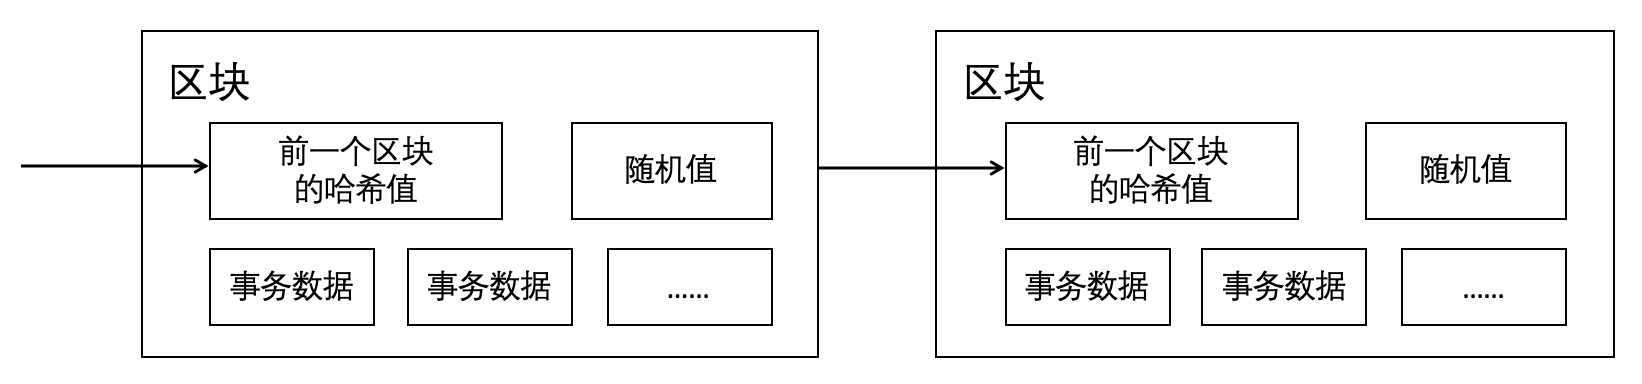
\includegraphics [width=0.75,height=2.5]{figures/hashchain.png}
\caption{Proposed Secure Systolic Montgomery modular MultiplierArchitecture}
\label{fig:hashchain}
\end{figure}

区块链系统各节点通过一定的共识机制选取具有打包交易权限的区块节点,该节点需要将新区块的前一个区块的哈希值、当前时间戳、一段时间内发生的有效交易及其梅克尔树根植等内容打包成一个区块,向全网广播。对原数据的任何改动,都将生成不同的消息摘要,这就使得该算法充分保证原数据的完整性。正是由于上述重要特性,哈希算法被广泛应用于生成和验证数字签名、消息认证码、随机数产生、错误校正与检测等领域。

\subsection{非对称加密体制和电子签名}

密码体制分为对称密码体制和非对称密码体制。

图7  密码体制的基本模型

消息发送者从密钥源得到密钥,通过加密算法对消息进行加密得到密文;接收者收到密文后,利用从密钥源得到的密钥,通过解密算法对密文进行解密,得到原始消息。
在对称密码体制中,解密算法是加密算法的逆算法。也就是说,加解密过程使用的密钥具有唯一性,解密方必须事先知道加密密钥。这使得对称加密体制具有算法公开、加密速度快、加密效率高的优势。另外,随着加密用户增加,密钥数量呈几何级数增长,密钥管理成本高,对称密码体制在分布式网络的应用受到阻碍。目前,广泛应用的对称密码体制有DES、3DES、国际数据加密算法(International Data Encryption Algorithm, IDEA)、高级数据加密标准(Advanced Encryption Standard, AES)和国内的SM1、SM4等。
 
图 8  对称密码体制加密流程

在非对称密码体制中,公钥和私钥的配对使用是明文加解密的关键。公钥用于加密明文,私钥用于解密密文。若发信方(加密者)想发送只有收信方(解密者)才允许解读的信息,发信方必须首先知道收信方公钥,并利用此公钥加密;该份密文用且仅能用收信方的私钥解密。由此可见,非对称密码体制拥有两个秘钥,且由公钥推出私钥在计算上是极为困难的,这也极大提高了数据加密安全性。公钥密码体制的建立,对密码学具有革命性的意义。目前,广泛应用的非对称密码体制有RSA、椭圆曲线密码(Elliptic Curve Cryptography, ECC)等。
 
图 9  公钥加密流程

正逐渐发展的数字签名便应用了公钥密码体制,公钥加密系统的加入,保证了数字签名的不可伪造性和不可抵赖性。数字签名跟手写签名的作用实质上是一样的,用来证明某个消息或者文件是本人发出/认同的。我国在2005年就已经施行《电子签名法》,确立了电子签名(包括但不限于数字签名)的法律效力。
常见的签名算法有RSA,DSA,ECDSA,其中RSA是实现数字签名最简单的公钥加密算法。RSA既可以用公钥加密然后私钥解密,也可以用私钥加密然后公钥解密,这是它的对称性。因为RSA中的每一个公钥都有唯一的私钥与之对应,任一公钥只能解开对应私钥加密的内容。
这样,如果你生成了一对RSA密钥,你把公钥公布出去,并告诉全世界人这个公钥是你的。之后你只要在发送的消息,比如“abcd”,后面加上用私钥加密过的密文,其他人拿公钥解密,看解密得到的内容是不是“abcd”就可以知道这个“abcd”是不是你发的。其他人没有对应的私钥,没法生成公钥可以解密的密文,所以是不可伪造的。又因为公钥对应的私钥只有一个,所以只要能成功解密,那么发消息的一定是你,不会是其他人,所以是不可抵赖的。
数字签名的用途很多,最常见的用处就是用来认证一个网站的身份,比如百度主页的数字签名证书。除此之外,代码签名也是其重要的用途。如果Windows上的可执行程序来源于正规公司,那么通常它会有代码签名,用于确保其来源可靠且未被篡改。
	
\subsection{布尔过滤器}

传统验证数据是否存在集合中的算法都会随着集合的数量增加而增加,为了解决这一问题,布尔过滤器利用哈希算法的输出长度固定性,利用固定长度的数组存储集合,对元素进行哈希变换,然后根据输出找到对应下标并在数组中记录或查询。为了解决不同输入映射到同一下标的问题,通常采用多个哈希函数共同确认。布尔过滤器具有很好的空间和时间效率,被用来检测一个元素是不是集合中的一个成员。在以太坊项目中,布尔过滤器被用于检测交易是否在给定区块中,便于用户快速检索特定交易的存储位置。和布尔过滤器类似,密码累加器也用于高效验证数据的存在性,后者还可以提供高效安全的存在性证明。在零币项目中,密码累加器用于存储用户加入的未花费代币的对应编码,当用户使用时,其他用户可以高效验证花费的代币是否存在。

同态加密使用户可以对加密数据不需要解密成明文,直接进行有效处理。对经过同态加密的数据进行处理得到一个输出,将这一输出进行解密,其结果与用同一方法处理未加密的原始数据得到的输出结果是一样的。在ZeroCash项目中主要用于隐藏事务中的核心隐私数据,构造零知识证明,在提供数据隐私性的前提下保障隐私数据的可验证和可信性。

安全多方计算的研究主要是针对无可信第三方的情况下,如何安全地计算一个约定函数,并且保障每一个输入数据的隐私性。安全多方计算用于构造零知识证明所需的可信启动参数,通过多方参与计算防止任何一方作恶。

目前,许多密码学技术仍在探索状态,区块链系统还需要研究如何更好地运用现有的密码学技术,另一方面,直接运用现有的密码学技术还存在性能、安全性等方面的不足之处,需要进一步研究密码学技术在区块链系统中的运用以及合理改进,提供更多的密码学性质以及提升系统性能。
